%%%%%%%%%%%%%%%%%%%%%%%%%%%%%%%%%%%%%%%%%%%%%%%%%%%%%%%%%%%%%%%%%%%%%%%%%%%%%%%%
% Uncertainties and Results:
%%%%%%%%%%%%%%%%%%%%%%%%%%%%%%%%%%%%%%%%%%%%%%%%%%%%%%%%%%%%%%%%%%%%%%%%%%%%%%%%
\chapter{Statistical Analysis, Uncertainties and Results}
\label{statAnalysis_uncerts_results}
%%%%%%%%%%%%%%%%%%%%%%%%%%%%%%%%%%%%%%%%%%%%%%%%%%%%%%%%%%%%%%%%%%%%%%%%%%%%%%%%
The results and their uncertainties obtained in this search are presented here.  Evidence in 
support of a \WR and \nul signal was sought in finite sized windows of $\Mlljj$, whose sizes 
were chosen to minimize the upper bound \WR cross section limit in the absence of a signal.  
Uncertainties that affected the background and signal estimates were measured in each $\Mlljj$ 
window.  The main uncertainties that affected the background estimate arose from limited event 
statistics in $e\mu$ data, and discrepancies between data and simulations in \DY-rich control 
regions.  The main uncertainties that affected the signal estimate came from luminosity and 
pileup measurements in data.  Additional sources of uncertainty existed and were measured, 
but had a smaller cumulative impact on the results.  Following uncertainty estimation, the 
results were obtained by comparing data, expected SM backgrounds and hypothetical 
\WR and \nul signals using the $\Mlljj$ distribution, and limits on the \WR cross section, 
$\mWR$ and $\mnul$ masses derived from data and expected backgrounds.

%%%%%%%%%%%%%%%%%%%%%%%%%%%%%%%%%%%%%%%%%%%%%%%%%%%%%%%%%%%%%%%%%%%%%%%%%%%%%%%%
% Statistical Analysis 
%%%%%%%%%%%%%%%%%%%%%%%%%%%%%%%%%%%%%%%%%%%%%%%%%%%%%%%%%%%%%%%%%%%%%%%%%%%%%%%%
\section{Statistical Analysis}
\label{sec:massWindows}
%%%%%%%%%%%%%%%%%%%%%%%%%%%%%%%%%%%%%%%%%%%%%%%%%%%%%%%%%%%%%%%%%%%%%%%%%%%%%%%%
The \WR and \nul signals considered in this search were characterized by $\Mlljj$ distributions 
that peaked at \mWR, and had tails that extended several hundred $\GeV$ below and above the 
peak.  The only other assumption made regarding the shape of signals in $\Mlljj$ was that 
the tails grew larger as \mWR increased, as shown in Figure \ref{fig:fig:signalShapesAfterSelection}.  
The general shape of \WR signals in the $\Mlljj$ distribution motivated the use of finite 
size $\Mlljj$ windows to search for evidence in support of LRS models.

\begin{figure}[btp]
	\centering
	\subfigure{
		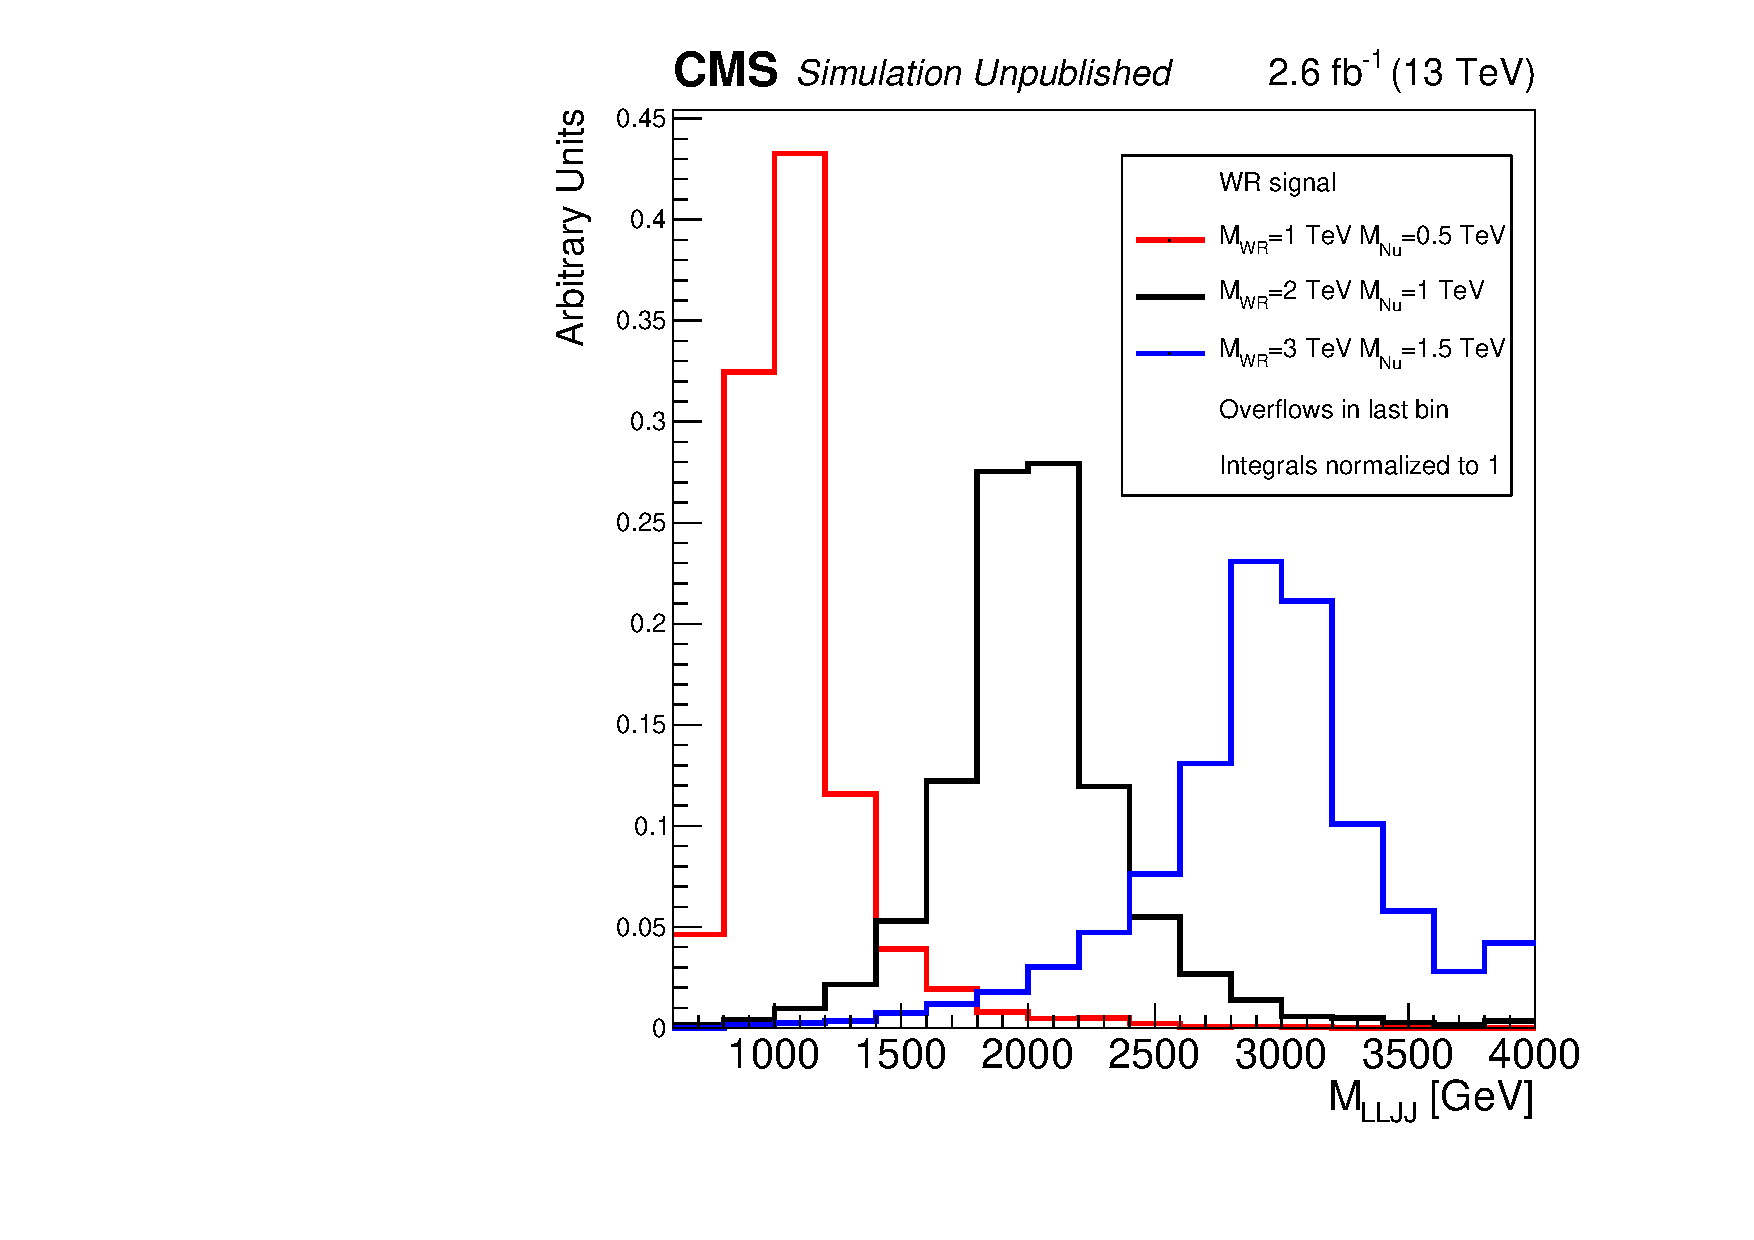
\includegraphics[width=0.45\textwidth]{figures/Mlljj_signalRegionCuts_severalWrSignals_EE.pdf}
	}
	\subfigure{
		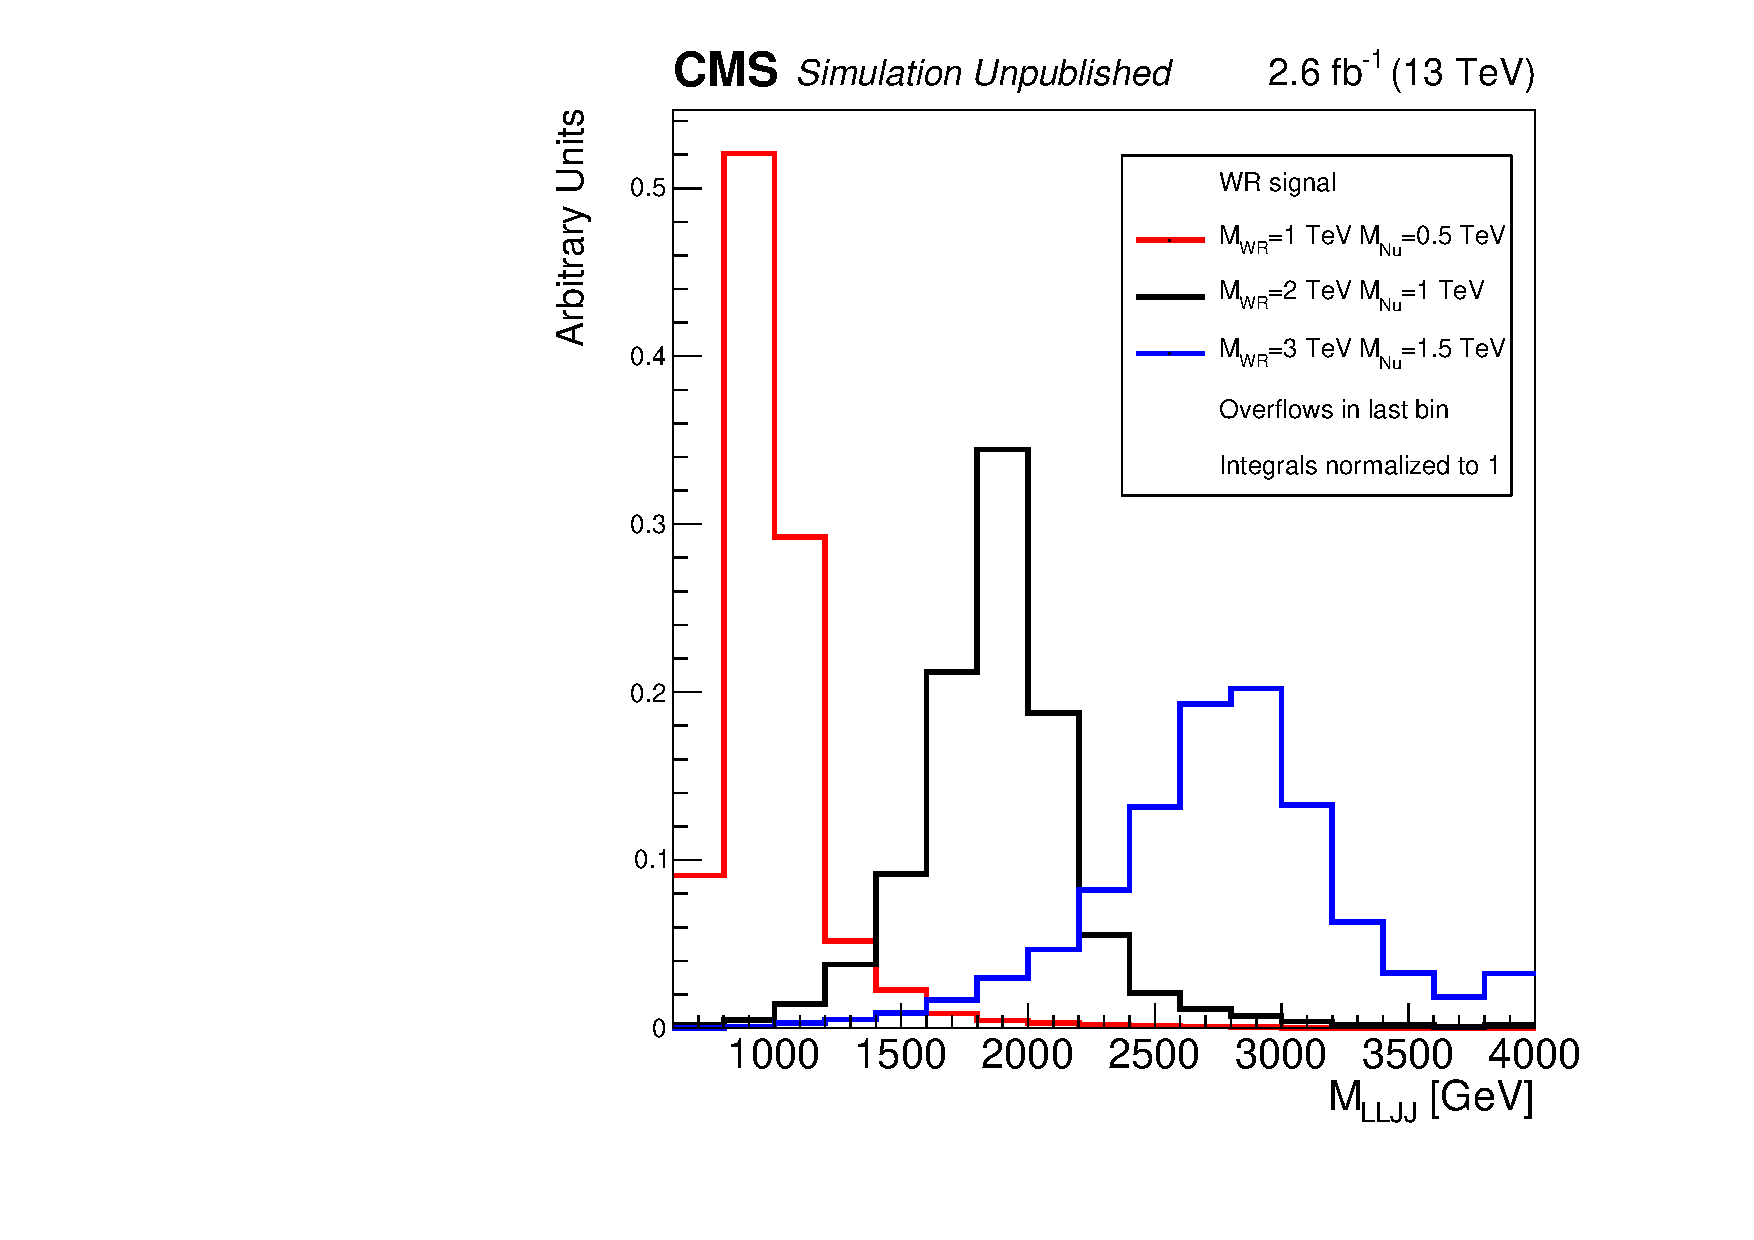
\includegraphics[width=0.45\textwidth]{figures/Mlljj_signalRegionCuts_severalWrSignals_MuMu.pdf}
	}
	\label{fig:signalShapesAfterSelection}
	\caption{$\Mlljj$ distribution after all selections for several \WR signal hypotheses in the $ee$ (left) and $\mu\mu$ (right) 
		channels.  The tails of the distribution grew as \mWR increased.}
\end{figure}

The SM backgrounds that passed the signal region selection were characterized by $\Mlljj$ 
distributions that decreased rapidly with increasing $\Mlljj$, whereas any \WR signal 
after the same selection appeared as an individual peak in the $\Mlljj$ distribution.  
This distinction motivated the division of the entire $\Mlljj > 600\GeV$ range into finite 
width $\Mlljj$ windows linked to specific \mWR hypotheses.  The optimal window size for each 
\mWR hypothesis was determined using the following procedure:

\begin{itemize}
	\item $\sim$150 $\Mlljj$ windows of different sizes were defined based on the expected width of the \WR $\Mlljj$ distribution.
	\item In each window:
	\begin{itemize}
		\item The number of expected signal events $A$ and all SM background events $B$ were calculated.
		\item A Poisson distribution was made with mean equal to $B$, and a random number $C$ representing 
			the number of measured events in the window was pulled from the Poisson distribution.
		\item Using the procedure described in Chapter \ref{sec:searchResults}, the probability that $C$ 
			was measured due to a fluctuation in $A$ and $B$ was calculated, and was rescaled into an 
			upper limit on the \WR cross section.  The size of fluctuations of $A$ and $B$ only depended 
			on their statistical uncertainties.
		\item The cross section limit calculation was repeated 300 times, and each time a new random 
			number $C$ was pulled from the Poisson distribution with mean $B$.  The median value of 
			all 300 limits was taken as the cross section upper limit for the window.
	\end{itemize}
	\item The window that minimized the \WR cross section upper limit was used with the \mWR hypothesis.
\end{itemize}

The $\Mlljj$ window optimization yielded the windows listed in Table \ref{tab:masscuts}.  The windows 
overlapped in $\Mlljj$ because one event with a unique $\Mlljj$ value was compatible with several 
\mWR hypotheses.  In each window the number of events observed in data, and expected from \WR 
signal and all SM backgrounds were counted.  In calculating the expected \WR signal events, only 
the \mWR hypothesis used to optimize the window was considered.  The effect of uncertainties on 
expected event estimates were calculated in each window using procedures described in the next 
section.

\begin{table}[h]
\caption{$\Mlljj$ window ranges that minimized the expected upper limit on the \WR cross section at different \mWR values.}
\label{tab:masscuts}
\centering
\begin{tabular}{|c|r@{ - }l|r@{ - }l|} \hline
\mWR (\GeV) & \multicolumn{4}{c|}{\Mlljj window (\GeV)}  \\\hline
& \multicolumn{2}{c|}{Electrons}  & \multicolumn{2}{c|}{Muons}  \\  \hline
 800  & 700       &  1100       &  700       &  1200      \\  \hline
1000  & 900       &  1300       &  900       &  1400      \\  \hline
1200  & 1100       &  1550       &  1100       &  1650      \\  \hline
1400  & 1250       &  1750       &  1300       &  1850      \\  \hline
1600  & 1450      &  2000       &  1500      &  2100      \\  \hline
1800  & 1600      &  2250       &  1600      &  2300      \\  \hline
2000  & 1850      &  2550       &  1850      &  2600      \\  \hline
2200  & 2000      &  2800       &  2000      &  2850      \\  \hline
2400  & 2150      &  3100       &  2150      &  3100      \\  \hline
2600  & 2250      &  3400       &  2300      &  3400      \\  \hline
2800  & 2350      &  3700       &  2400      &  3700      \\  \hline
3000  & 2500      &  4000       &  2500      &  3950      \\  \hline
3200  & 2550      &  4300       &  2700      &  4250      \\  \hline
3600  & 2700      &  4900       &  2900      &  4850      \\  \hline
3800  & 2750      &  5200       &  2950      &  5150      \\  \hline
4000  & 2800      &  5500       &  3000      &  5450      \\  \hline
4200  & 2800      &  5750       &  3100      &  5750      \\  \hline
4400  & 2850      &  6050       &  3150      &  6100      \\  \hline
4600  & 2850      &  6300       &  3150      &  6400      \\  \hline
4800  & 2850      &  6600       &  3200      &  6700      \\  \hline
5000  & 2900      &  6850       &  3200      &  7000      \\  \hline
5200  & 2900      &  7050       &  3200      &  7300      \\  \hline
5600  & 2900      &  7500       &  3200      &  7850      \\  \hline
5800  & 2950      &  7700       &  3200      &  8150      \\  \hline
6000  & 2950      &  7900       &  3200      &  8400      \\  \hline
\end{tabular}
\end{table}


%%%%%%%%%%%%%%%%%%%%%%%%%%%%%%%%%%%%%%%%%%%%%%%%%%%%%%%%%%%%%%%%%%%%%%%%%%%%%%%%
% Uncertainties 
%%%%%%%%%%%%%%%%%%%%%%%%%%%%%%%%%%%%%%%%%%%%%%%%%%%%%%%%%%%%%%%%%%%%%%%%%%%%%%%%
\section{Uncertainties}
\label{sec:uncertainties}
%%%%%%%%%%%%%%%%%%%%%%%%%%%%%%%%%%%%%%%%%%%%%%%%%%%%%%%%%%%%%%%%%%%%%%%%%%%%%%%%
In each window the estimated number of expected signal and background events were subject to 
many sources of uncertainty.  The sizes of these uncertainties were estimated in several ways, and 
when calculating the search results the effects of the uncertainties were included as percentage 
uncertainties on the expected number of events in each window.

The impact of uncertainties that affected lepton and jet selection was 
estimated simultaneously with the impact of the statistical uncertainty, but ignoring other 
uncertainties.  In a set of events, from data or simulations, that had a subset passing the full 
selection, varying the measured values of $\Et$ or $\pt$ and identification variables by their 
uncertainties resulted in the following:

\begin{itemize}
	\item Some events that failed the full selection without any uncertainty variations suddenly passed the 
		selection after varying the measured values.
	\item Some events that passed the full selection without any uncertainty variations suddenly failed the 
		selection after varying the measured values.
	\item Some events that passed the full selection without any uncertainty variations again passed the 
		selection after varying the measured values, but different leptons or jets were selected, and 
		as a result the events migrated to other $\Mlljj$ windows.
	\item Some events that passed the full selection without any uncertainty variations again passed the 
		selection after varying the measured values, the same leptons and jets were selected as if no 
		variations were applied, and the events fell in the same $\Mlljj$ windows.
	\item Some events that passed the full selection without any uncertainty variations again passed the 
		selection after varying the measured values, the same leptons and jets were selected as if no 
		variations were applied, but the energy variations moved the events to other $\Mlljj$ windows.
\end{itemize}

The magnitudes of lepton and jet uncertainties varied with lepton and jet kinematic variables, 
including energy and trajectory, and were estimated and validated independent of physics analyses.  
The impact of these uncertainties on estimates of expected background and signal events was 
determined by applying the following procedure\footnote{This procedure was reviewed and approved by the CMS Collaboration.} 
independently to simulated $\DY$ events, simulated $\WR \rightarrow \ell\ell jj$ events, and 
$e\mu$ events from data representing the top quark background:

\begin{itemize}
	\item For .
\end{itemize}




\begin{table}[ht]
	\caption{Magnitude of individual \emph{Category B} uncertainties for the $\MWR = 2.2\TeV$ hypothesis.  All
	uncertainties in percent of expected events.  Note the lepton uncertainty for Top backgrounds is the combination of electron and muon uncertainties, while for DY and \WR it is electron only or muon only.  All uncertainties obtained by throwing 3200 toys.}
  \label{tab:catBUncertaintiesOneMassBin}
  \centering
    \begin{tabular}{c|c|c}
%      \hline
		Uncertainty                  & eejj magnitude (\%) & $\mu\mu$jj magnitude (\%)  \\
      \hline
	  \WR lepton energy scale and resolution, ID and iso & $1$ & $3$ \\ 
	  \WR jet energy scale and resolution & $1$ & $1$ \\ 
	  DY lepton energy scale and resolution, ID and iso & $4$ & $7$  \\
	  DY jet energy scale and resolution & $14$ & $11$  \\
	  Top lepton energy scale and resolution, ID and iso & $8$ & $8$ \\
	  Top jet energy scale and resolution & $2$ & $2$  \\
  \hline
  \end{tabular}
\end{table}



%%%%%%%%%%%%%%%%%%%%%%%%%%%%%%%%%%%%%%%%%%%%%%%%%%%%%%%%%%%%%%%%%%%%%%%%%%%%%%%%
% Results
%%%%%%%%%%%%%%%%%%%%%%%%%%%%%%%%%%%%%%%%%%%%%%%%%%%%%%%%%%%%%%%%%%%%%%%%%%%%%%%%
\section{Results}
\label{sec:searchResults}
%describe how limits are calculated with and without syst uncertainties before showing results
%when explaining limit calculation procedure without syst uncertainties, refer back to 
%Chapter \ref{sec:massWindows}

%%%
%from statistical.tex file of AN
%The probability of the observed number of events being produced by a combination of background and signal with a cross section ($x$) is calculated using the Bayesian approach with the \emph{combine} tool with flat prior. 
%The exclusion limit on the cross section ($x$) is defined as the value for which the posterior likelihood reaches 95\% of the total area under the curve.
%This is repeated for each mass hypothesis.
%
%In order to take into account the uncertainties, pseudo-experiments are performed by the \combine tool varying the expected number of events from signal and background according to the uncertainties as described in the following section. The median of the distribution of the excluded cross section produced by pseudo-experiments and the intervals containing 68\% and 95\% of the pseudo-experiments are then quoted in the ``expected'' limits.
%%%


%%%%%%%%%%%%%%%%%%%%%%%%%%%%%%%%%%%%%%%%%%%%%%%%%%%%%%%%%%%%%%%%%%%%%%%%%%%%%
